\documentclass[10pt,handout]{beamer}

\usetheme{Madrid}
\usecolortheme{default}

% Base packages
%\usepackage{helvet}
\usepackage{amsthm,graphicx,xcolor,natbib,booktabs,tabularx,mathtools,subcaption}
\usepackage{unicode-math,mathrsfs}
\usepackage{amsmath,amssymb}
\usepackage{tikz,pgfplots}
\usetikzlibrary{arrows.meta, positioning, quotes}

\usepackage[cache=false]{minted}
\renewcommand{\theFancyVerbLine}{\sffamily\textcolor[rgb]{0.5,0.5,1.0}{\scriptsize\oldstylenums{\arabic{FancyVerbLine}}}}
\definecolor{bg}{rgb}{.95,.95,.95}

% Font settings
\renewcommand{\familydefault}{\sfdefault}

% TikZ libraries
\usetikzlibrary{calc,positioning,backgrounds,decorations.pathreplacing}
\pgfplotsset{compat=1.14}

% Colors
\definecolor{deepblue}{RGB}{42,39,155}
\definecolor{lightpink}{RGB}{255,240,240}
\definecolor{lightgreen}{RGB}{240,255,240}
\definecolor{lightyellow}{RGB}{255,255,240}
\definecolor{codegray}{RGB}{245,245,245}
\definecolor{codegreen}{rgb}{0,0.6,0}
\definecolor{codepurple}{rgb}{0.58,0,0.82}

% Beamer settings
\setbeamercolor{title}{fg=white,bg=deepblue}
\setbeamercolor{frametitle}{fg=white,bg=deepblue}
\setbeamercolor{section in head/foot}{fg=white,bg=deepblue}

\setbeamertemplate{footline}[text line]{%
  \parbox{\linewidth}{\vspace*{-8pt}
  %\hfill\href{https://github.com/chang-ye-tu/fin}{https://github.com/chang-ye-tu/fin}
    \hfill
   \insertframenumber~/ \inserttotalframenumber}}
\setbeamertemplate{navigation symbols}{}%[only frame symbol]

\definecolor{foo}{rgb}{.2,.2,.7}
\AtBeginSection[]{
  \begin{frame}
  \vfill
  \centering
  \begin{beamercolorbox}[sep=8pt,center,shadow=true,rounded=true]{section page}
    \usebeamerfont{title}%
    {\color{foo} \insertsectionhead}\par%
  \end{beamercolorbox}
  \vfill
  \end{frame}
}

% https://tex.stackexchange.com/questions/30423/bibliography-in-beamer
\setbeamertemplate{bibliography entry title}{}
\setbeamertemplate{bibliography entry location}{}
\setbeamertemplate{bibliography entry note}{}

\usepackage{dsfont} % indicator function \mathds{1}
\DeclareMathOperator\indc{\mathds{1}}
\newcommand{\ds}{\displaystyle}
\newcommand{\ie}{\;\Longrightarrow\;}
\newcommand{\ifff}{\;\Longleftrightarrow\;}
\newcommand{\mi}{\mathrm{i}}
\DeclareMathOperator*{\dom}{dom}
\DeclareMathOperator*{\codom}{codom}
\DeclareMathOperator*{\ran}{ran}
\newcommand{\floor}[1]{\lfloor #1 \rfloor}
\newcommand{\ceil}[1]{\lceil #1 \rceil}
\newcommand{\Set}[2]{\big\{ \ #1\ \big|\ #2\ \big\}}
\newcommand{\pdiff}[2]{\frac{\partial\hfil#1\hfil}{\partial #2}}
\newcommand{\vx}{\symbfup{x}}
\newcommand{\vd}{\symbfup{d}}
\newcommand{\vg}{\symbfup{g}}
\newcommand{\vH}{\symbfup{H}}
\newcommand{\va}{\symbfup{a}}
\newcommand{\vb}{\symbfup{b}}
\newcommand{\vbb}{\symbfup{\beta}}
\newcommand{\vS}{\symbfup{S}}
\newcommand{\vR}{\symbfup{R}}
\newcommand{\vV}{\symbfup{V}}
\newcommand{\ve}{\symbfup{e}}
\newcommand{\vr}{\symbfup{r}}
\newcommand{\vZero}{\symbfup{0}}

\DeclareMathOperator\prb{{\sf P}}
\DeclareMathOperator\expc{{\sf E}}
\DeclareMathOperator\var{var}
\DeclareMathOperator\cov{cov}
\DeclareMathOperator\cor{cor}
\DeclareMathOperator*{\argmax}{\arg\!\max}
\DeclareMathOperator*{\argmin}{\arg\!\min}
\DeclareMathOperator*{\im}{Im}
\DeclareMathOperator*{\re}{Re}
\DeclareMathOperator*{\conv}{conv}
\DeclareMathOperator*{\proj}{proj}
\DeclareMathOperator*{\tr}{tr}
\DeclareMathOperator*{\diag}{diag}
\DeclareMathOperator*{\epi}{epi}
\DeclareMathOperator*{\dist}{dist}
\DeclareMathOperator*{\inte}{int}
\DeclareMathOperator*{\relint}{relint}

\theoremstyle{definition}
\newtheorem*{dfn}{Definition}
\newtheorem*{prp}{Property}
\newtheorem*{thm}{Theorem}
\newtheorem*{ex}{Example}
\newtheorem*{prob}{Problem}
\newtheorem*{sol}{Solution}
\newtheorem*{prf}{Proof}
\usepackage{nicefrac}
\usepackage{multicol}

\newcommand\scalemath[2]{\scalebox{#1}{\mbox{\ensuremath{\displaystyle #2}}}}

\title{Options \& Derivatives}
\author{}
\date{}

\begin{document}

\begin{frame}
\titlepage
\end{frame}

%\subsection*{Outline}
%\begin{frame}
%  \tableofcontents
%\end{frame}

\begin{frame}{The One Period Model}
  \begin{itemize}
    \item time $t$: $t=0, 1$ 
    \item (deterministic) bond $B_t$: $\ds B_0 = 1,\;B_1 = 1 + R$
    \item (stochastic) stock $S_t$: $\ds S_0 = s > 0, \; S_1 = \begin{cases} s\cdot u & \text{with prob. } p_u\\ s\cdot d & \text{with prob. } p_d \end{cases} \equiv s\,Z:\;$ $u > d$, $p_u + p_d = 1$.
    \item The value $V_t^h$ of the portfolio $h=(x, y),\,x, y\in\mathbb{R}$ at time $t$: $\ds V_t^h = x\,B_t + y\,S_t$ --- $\ds V_0^h = x + y\,s,\; V_1^h = x(1 + R) + y\,s\,Z$
    \item Arbitrage portfolio $h$: $V_0^h=0$, $V_1^h>0$ with prob. $1$.
  \end{itemize}
  \begin{figure}[!htbp]
    \centering
    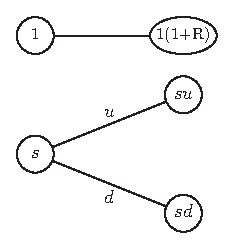
\includegraphics[scale=0.9,page=1]{fig/note08/bjork.pdf}
    \caption{Asset Dynamics of One Period Model.}
    \label{fig:bn1}
  \end{figure}
\end{frame}

\begin{frame}{Portfolios and Arbitrage I}
  \begin{thm}
    The one period model is arbitrage free $\ifff$ $\ds u\geqslant 1+R \geqslant d$.
  \end{thm}
  \begin{prf}
    ($\Longrightarrow$)
    \begin{itemize}
      \item Suppose $u\geqslant 1+R \geqslant d$ does not hold, then $1 + R > u$ or $d > 1 + R$.
      \item If $1 + R > u$, then $s(1 + R) > s\,u$ and a priori $s(1+R) > s\,d$.
      \item Consider $h = (s, -1)$, then $V_0^h = s\cdot 1 + (-1)\cdot s = 0$, $V_1^h = s(1 + R) - s\cdot Z >0$, an arbitrage.
      \item If $d > 1 + R$, then $s\,d > s(1 + R)$ and a priori $s\,u > s(1 + R)$.
      \item Consider $h = (-s, 1)$, then $V_0^h = (-s)\cdot 1 + 1\cdot s = 0$, $V_1^h = -s(1 + R) + s\cdot Z > 0$, an arbitrage.
    \end{itemize}
  \end{prf}
\end{frame}
\begin{frame}{Portfolios and Arbitrage II}
  \begin{thm}
    The one period model is arbitrage free $\ifff$ $\ds u\geqslant 1+R \geqslant d$.
  \end{thm}
  \begin{prf}
    ($\Longleftarrow$)
    \begin{itemize}
      \item Arbitrage $h = (x, y)$: $V_0^h = 0$.
      \item $ x + s\cdot y = 0\ie x= -s\cdot y$. 
      \item $\ds V_1^h = \begin{cases}y\,s\big(u - (1 + R)\big),&\; Z=u \\ y\,s\big(d - (1 + R)\big),&\; Z=d\end{cases}$
      \item If $y > 0$: from $\ds V_1^h > 0$ $\ie$ $u > 1 + R$ and $d > 1 + R$; a contradiction.
      \item If $y < 0$: from $\ds V_1^h > 0$ $\ie$ $u < 1 + R$ and $d < 1 + R$; a contradiction.
    \end{itemize}
  \end{prf}
\end{frame}

%\begin{thm}
%  $\ds \text{ No arbitrage }\ifff u\geqslant 1+R \geqslant d$
%\end{thm}

\begin{frame}{Risk-Neutral / Martingale Measure and Probabilities}
  \begin{itemize}
    \item Observation: $u\geqslant 1+R \geqslant d$ $\ie$ $1 + R$ is a convex combination of $u$ and $d$  
    \item $\ds\exists\,q_u, q_d \geqslant 0,\,\,q_u+q_d = 1\;\text{ s.t. }\; 1 + R = q_u\cdot u + q_d\cdot d$
    \item Define a new probability measure $Q$ and the associated expectation $\expc^Q$ s.t. 
      \begin{align*}
        &Q(Z = u) = q_u,\quad Q(Z = d) = q_d \\
        &\frac{1}{1+R}\expc^Q S_1 = \frac{1}{1+R}(q_u\cdot s\,u + q_d\cdot s\,d) = \frac{1}{1+R}\cdot s(1+R) = s
      \end{align*}
  \end{itemize}
  \begin{dfn}
    \begin{itemize}
      \item \textbf{Risk-Neutral / Martingale Measure}: A measure $Q$ satisfies $\ds S_0 = \frac{1}{1+R}\expc^Q S_1$.
      \item \textbf{Martingale Probabilities}: $\ds q_u = \frac{(1+R)-d}{u-d}, \;q_d = \frac{u-(1+R)}{u-d}$
    \end{itemize}
  \end{dfn}
\end{frame}

\begin{frame}{Contingent Claims I}
  \begin{dfn}
    \begin{itemize}
      \item A \textbf{contingent claim} $X$ is of the form $X=\Phi(Z)$
      \item Stochastic $Z$ with \textbf{contract function} $\Phi(\cdot)$
      \item \textbf{Price} of $X$ at time $t$: $\Pi(t; X)$
    \end{itemize}
  \end{dfn}
  \begin{figure}[!htbp]
    \centering
    \includegraphics[scale=.9,page=2]{fig/note08/bjork.pdf}
    \caption{The Contingent Claim.}
    \label{fig:bn2}
  \end{figure}
\end{frame}

\begin{frame}{Contingent Claims II}
  \begin{example}[European Call Option with Strike $K$]
    Assume $s\, u > K > s\, d$. At $t=1$, 
    \begin{itemize}
      \item Exercise the option if $S_1 > K$.
        \begin{itemize}
          \item Pay $K$ to get the stock and sell it at $s\,u$, thus making net profit $s\,u-K$.
        \end{itemize}
      \item Do nothing if $S_1 < K$.
    \end{itemize}
    \begin{align*}
      X = \begin{cases}s\,u - K, & Z=u \\ 0,  & Z=d\end{cases}, \quad\begin{cases}\Phi(u) = s\, u - K \\ \Phi(d) = 0\end{cases}
    \end{align*}
  \end{example}
  \begin{dfn}
    \begin{itemize}
      \item A contingent claim $X$ is said to be \textbf{reachable} if there exists a portfolio $h$ such that $V_1^h = X$ with probability 1; this portfolio $h$ is called a \textbf{hedging} or \textbf{replicating} portfolio. 
      \item If all claims can be replicated we say the market is \textbf{complete}.
    \end{itemize}
  \end{dfn}
\end{frame}

\begin{frame}{Contingent Claims III}
\begin{thm}[Pricing Principle]
  If a claim $X$ is reachable with replicating portfolio $h$, then the ``reasonable'' price of $X$ is given by $\ds\Pi(t; X) = V_t^h, \; t=0, 1.$
\end{thm}

\begin{thm}
  An arbitrage free one period model is complete.
\end{thm}

\begin{prf}
  Fixed any $\Phi(\cdot)$, show that $\exists\,h=(x, y)$ s.t.
  \begin{align*}
    V_1^h = \begin{cases}\Phi(u)\quad Z=u,\\ \Phi(d)\quad Z=d.\end{cases}\!\!\!\!\Longrightarrow x(1+R) + y\,s\,u = \Phi(u), \; x(1+R) + y\,s\,d = \Phi(d).
  \end{align*}
  Solve for $x, y$: $\ds x = \frac{1}{1+R}\,\frac{u\Phi(d)-d\,\Phi(u)}{u-d},\quad y = \frac{1}{s}\,\frac{\Phi(u)-\Phi(d)}{u-d}$.
\end{prf}
\end{frame}

\begin{frame}{Risk Neutral Valuation}
  \begin{itemize}
    \item From Pricing Principle ($\Pi(t; X) = V_t^h,\, t=0,1$)
      \begin{align*}
        \Pi(0; X) &= V_0^h = x + s\,y \\
                  &= \frac{1}{1+R}\cdot\frac{u\Phi(d)-d\,\Phi(u)}{u-d} + s\cdot\frac{1}{s}\cdot\frac{\Phi(u)-\Phi(d)}{u-d} \\
                  &= \frac{1}{1+R}\left\{\frac{(1+R)-d}{u-d}\,\Phi(u) + \frac{u-(1+R)}{u-d}\,\Phi(d)\right\}\\
                  &= \frac{1}{1+R}\left\{q_u\,\Phi(u) + q_d\,\Phi(d)\right\} \equiv \frac{1}{1+R}\expc^Q X
      \end{align*}
  \end{itemize}
  \begin{thm}[The Risk Neutral Valuation Principle]
    If the one period binomial model is arbitrage-free, then the price of $X$ is $\ds\Pi(0; X) = \frac{1}{1+R}\expc^Q X$.
  \end{thm}
\end{frame}

\begin{frame}{The Multiperiod Model}
  \begin{itemize}
    \item time $t$: $t=0, 1, 2, \ldots, T$ 
    \item (deterministic) bond $B_t$ with $\ds B_0 = 1,\; B_{n+1} = (1 + R)B_n$
    \item (stochastic) stock $S_t$ with $\ds S_0 = s > 0,\; S_{n+1} = Z_n\,S_n$ where $Z_0, Z_1, Z_2,\ldots, Z_{T-1}$ are iid with $\ds\prb(Z_n=u) = p_u,\;\prb(Z_n=d) = p_d$
  \end{itemize}
  \begin{figure}[!htbp]
    \centering
    \includegraphics[scale=.75,page=3]{fig/note08/bjork.pdf}
    \vspace{-3mm}
    \caption{Asset Dynamics of Multiperiod Model: ``Recombining'' Tree.}
    \label{fig:bn3}
  \end{figure}
\end{frame}

\begin{frame}{Portfolios and Arbitrage}
\begin{dfn}
  The portfolio $h_t \equiv (x_t, y_t)$; The value $V_t^{h_t}$ of portfolio $h_t$ at time $t$ is $\ds V_t^{h_t} = x_t\,B_t + y_t\,S_t$.
\end{dfn}
\begin{itemize}
  \item Hereafter we write $V_t^h$ instead of the cumbersome $V_t^{h_t}$. 
  \item $x_t$ is the amount which we invest in the bank at time $t-1$ and keep until $t$.
\end{itemize}
\begin{dfn}
  Self-financing portfolio $h_t=(x_t, y_t)$: $\ds x_t\,(1 + R) + y_t\,S_t = x_{t+1} + y_{t+1}\,S_t,\quad\forall t = 0, 1, \ldots, T-1.$
\end{dfn}
\end{frame}

\begin{frame}{Contingent Claims}
\begin{dfn}
  \begin{itemize}
    \item Arbitrage: there exists a self-financing portfolio $h_t$ with $\ds V_0^h = 0$, $\prb(V_T^h\geqslant 0) = 1$, $\ds\prb(V_T^h>0) > 0$.
    \item A contingent claim $X$ is said to be \textbf{reachable} if there exists a self-financing portfolio $h$ such that $V_T^h = X$ with probability 1; this portfolio $h$ is called a \textbf{hedging} or \textbf{replicating} portfolio. 
    \item If all claims can be replicated we say the market is \textbf{complete}. 
  \end{itemize}
\end{dfn}

\begin{thm}[Pricing Principle]
  If a claim $X$ is reachable with replicating (and self-financing) portfolio $h$, then the ``reasonable'' price process of $X$ is given by $\ds \Pi(t; X) = V_t^h, \; t=0, 1, 2, \ldots T$.
\end{thm}

\begin{thm}
  An arbitrage-free multiperiod model is complete.
\end{thm}
\end{frame}
  
\begin{frame}
  \begin{thm}[Binomial Algorithms]
    \begin{itemize}
      \item Given a contingent claim $X=\Phi(S_T)$; let $V_t(k)$ denotes the value of the replicating portfolio at node $(t, k)$, then $V_t(k)$ is computed recursively by 
        \begin{align*}
          V_T(k) &= \Phi(s\,u^k\,d^{T-k}) \\
          V_t(k) &= \frac{1}{1+R}\left\{q_u\,V_{t+1}(k+1) + q_d\,V_{t+1}(k)\right\}
        \end{align*}
      \item The martingale probabilities $q_u, q_d$ are $\ds q_u = \frac{(1+R)-d}{u-d}$, $\ds q_d = \frac{u-(1+R)}{u-d}$
      \item The replicating portfolio $h_t = (x_t, y_t)$ is \vspace{-3mm}
        \begin{align*}
          x_t(k) = \frac{1}{1+R}\,\frac{u\,V_t(k)-d\,V_t(k+1)}{u-d}, \quad y_t(k) = \frac{1}{S_{t-1}}\,\frac{V_t(k+1)-V_t(k)}{u-d}
        \end{align*}
      \item The arbitrage-free price of a contingent claim $X$ at $t=0$ is \vspace{-3mm} 
    \begin{align*}
      \Pi(0;X) = \frac{1}{(1 + R)^T}\expc^Q X = \frac{1}{(1 + R)^T}\cdot\sum_{k=0}^T\binom{T}{k}q_u^k\,q_d^{T-k}\Phi(s\,u^k\,d^{T-k})
    \end{align*}
    \end{itemize}
  \end{thm}
\end{frame}

\begin{frame}
  \begin{example}
    Given $T=3, S_0=80, K=80, u=1.5, d=0.5, p_u=0.6, p_d=0.4, R=0$, compute the European call option price and the replicating portfolio of each node.
  \end{example}
  \begin{figure}
    \centering
    \includegraphics[scale=.9,page=4]{fig/note08/bjork.pdf}
    \caption{Asset Dynamics of the Example.}
  \end{figure}  
\end{frame}

\begin{frame}
  \begin{figure}[!htbp]
    \centering
    \includegraphics[scale=1,page=5]{fig/note08/bjork.pdf}
    \caption{Payoff at the End of Terms.}
  \end{figure}
\end{frame}

\begin{frame}
  \begin{figure}[!htbp]
    \centering
    \includegraphics[scale=1,page=7]{fig/note08/bjork.pdf}
    \caption{Iterated Computation of $\ds\Pi(t;X):\;$ $\ds\Pi(t-1; X)\equiv\frac{1}{1+R}\expc^Q\{\Pi(t; X)\}$.} %$\;\ds = \frac{1}{1+R}\left\{q_u\Phi(u) + q_d\Phi(d)\right\}$}
  \end{figure}
\end{frame}

\begin{frame}
  \begin{figure}[!htbp]
    \centering
    \includegraphics[scale=1,page=9]{fig/note08/bjork.pdf}
    \caption{The Completed $\Pi(t; X)$.} 
  \end{figure}
\end{frame}

\begin{frame}
  \begin{figure}[!htbp]
    \centering
    \includegraphics[scale=1.05,page=10]{fig/note08/bjork.pdf}
    \caption{Replicating $h_t=(x_t, y_t):\;$ $x_t(k) = \frac{1}{1+R}\,\frac{u\,V_t(k)-d\,V_t(k+1)}{u-d}$, $y_t(k) = \frac{1}{S_{t-1}}\,\frac{V_t(k+1)-V_t(k)}{u-d}$}
  \end{figure}
\end{frame}

\begin{frame}
  \frametitle{Algorithmic Considerations}
    \begin{align*}
      \Pi(0;X)=\frac{1}{(1 + R)^T}\cdot\sum_{k=0}^T\binom{T}{k}q_u^k\,q_d^{T-k}\Phi(s\,u^k\,d^{T-k})
    \end{align*}
    For big $T$ the formula can't be directly used because of the binomial coefficient
    \begin{align*}
      V_T(k) = \Phi(s\,u^k\,d^{T-k}), \quad V_t(k) = \frac{1}{1+R}\left\{q_u\,V_{t+1}(k+1) + q_d\,V_{t+1}(k)\right\}
    \end{align*}
  \begin{figure}
    \includegraphics[width=.45\textwidth,page=2]{fig/note08/gilli.pdf}
    \includegraphics[width=.45\textwidth,page=3]{fig/note08/gilli.pdf}
    %\caption{Vector Update} 
  \end{figure}
\end{frame}

\begin{frame}[fragile]{Python Code Illustration: Common Parts}
  \begin{minted}{python}
  import numpy as np
  
  S0 = 80; r = 0; K = 80; u = 1.5; d = 0.5; 
  q = (1 - d) / (u - d); M = 3; 
  df = 1     # discount factor per time interval
  # exhibit stock paths
  S = np.zeros((M + 1, M + 1), dtype=np.float)  
  S[0, 0] = S0
  for j in range(1, M + 1, 1):
      for i in range(j + 1):
          S[i, j] = S[0, 0] * (u ** (j - i)) * (d ** i)
  \end{minted}
\end{frame}
  
\begin{frame}[fragile]{Python Codes: Traditional Loops}
  \begin{minted}[fontsize=\small]{python}
  iv = np.zeros((M + 1, M + 1), dtype=np.float); z = 0  # inner values
  for j in range(0, M + 1, 1):
      for i in range(z + 1):
          iv[i, j] = round(max(S[i, j] - K, 0), 8)
      z += 1
  
  pv = np.zeros((M + 1, M + 1), dtype=np.float)         # present values
  pv[:, M] = iv[:, M]
  z = M + 1
  for j in range(M - 1, -1, -1):
      z -= 1
      for i in range(z):
          pv[i, j] = (q * pv[i, j + 1] + (1 - q) * pv[i + 1, j + 1]) * df
  \end{minted}
\end{frame}

\begin{frame}{Python Codes: Vectorized Loops}
  \inputminted[fontsize=\footnotesize,linenos=true]{python}{fig/note08/binomial_vec.py}
\end{frame}

\begin{frame}
  \begin{ex}
  An investor purchases a nonindivident-paying stock and writes a $t$-year, European call option for this stock, with call premium $C$.The stock price at time of purchase and strike price are both $K$. Assume that there are no transaction costs. The risk-free annual force of interest is a constant $r$. Let $S$ represent the stock price at time $t$, $S > K$. What is the investor's profit at expiration?
  \end{ex}
  \begin{sol}
    The time $0$ investment is $S_0 - C = K - C$ and the time $t$ payoff is $S - (S - K)_+ = K$ for $S > K$. The profit at expiration is $K - (K - C)e^{rt}$.
  \end{sol}
\end{frame}

\begin{frame}
  \begin{ex}
    Stock A has the following characteristics:
    \begin{itemize}
      \item The current price is $40$.
      \item The price of a 35-strike 1-year European call option is 9.12.
      \item The price of a 40-strike 1-year European call option is 6.22.
      \item The price of a 45-strike 1-year European call option is 4.08.
    \end{itemize}
    The annual risk-free interest rate is 8\%. Let $S$ be the price of the stock one year from now. All call positions being compared are long. Determine the range of $S$ such that the 45-strike call produces a higher profit than the 40-strike call but a lower profit than the 35-strike call.
  \end{ex}
\end{frame}

\begin{frame}
  \begin{sol}
    Denote by $p_K$ the profit of a $K$-strike 1-year European call. We first express each $p_K$ in terms of $S$:
    \begin{align*}
      p_{35} &= (S - 35)_+ - 9.12\cdot 1.08 = (S - 35)_+ - 9.8496 \\
      p_{40} &= (S - 40)_+ - 6.22\cdot 1.08 = (S - 40)_+ - 6.7176 \\
      p_{45} &= (S - 45)_+ - 4.08\cdot 1.08 = (S - 45)_+ - 4.4064 
    \end{align*}
    To find the range for $S$ such that $p_{40} < p_{45} < p_{35}$, consider the followings:
    \begin{itemize}
      \item If $S < 35$ then all the $(\cdot)_+$ vanish, we have $p_{35} < p_{40} < p_{45}$, a contradiction. 
      \item If $35 \leqslant S < 40$, then $p_{35} = S - 44.8496$, $p_{40} = - 6.7176$, $p_{45} = -4.4064$. To make $p_{35} > p_{45}$, $S - 44.8496 > -4.4064$ $\ie$ $S > 40.4432$, a contradiction. 
      \item If $40 \leqslant S < 45$, then $p_{35} = S - 44.8496$, $p_{40} = S - 46.7176$, $p_{45} = -4.4064$. To make $p_{35} > p_{45}$, $S - 44.8496 > -4.4064$ $\ie$ $S > 40.4432$. To make $p_{45} > p_{40}$, $-4.4064 > S - 46.7176$ $\ie$ $42.3112 > S$. 
      \item If $S\geqslant 45$, $p_{40} < p_{45}$ $\ie$ $S - 46.71716 < S - 49.4064$ cannot hold.
    \end{itemize}
    So $40.4432 < S < 42.3112$.
  \end{sol}
\end{frame}

\begin{frame}
  \begin{ex}
    Investor A wrote a 104-strike 1-year call option whose price is 2. Investor B entered into a 1-year forward with a forward price of 105. The anually compounded risk-free interest rate is 5\%, and it turns out that investors A and B earn the same profit. What is the year 1 stock price? 
  \end{ex}
  \begin{sol}
    Equating the profits of the short call and long forward, 
    \begin{align*}
      2\cdot 1.05 - (S_1 - 104)_+ = S_1 - 105
    \end{align*}
    Consider the followings:
    \begin{itemize}
      \item If $S_1 < 104$ then $2\cdot 1.05 = S_1 - 105$ $\ie$ $S_1 = 107.1$, a contradiction to $S_1 < 104$. 
      \item If $S_1 \geqslant 104$ then $2\cdot1.05 - (S_1 - 104)  = S_1 - 105$ $\ie$ $S_1 = 105.55$. 
    \end{itemize}
    So $S_1 = 105.55$.
  \end{sol}
\end{frame}

\begin{frame}
  \begin{ex}
    For a certain stock, Investor A purchases a 45-strike call option while Investor B purchases a 135-strike put option. Both options
are European with the same expiration date. Assume that there are no transaction costs. If the final stock price at expiration is $S$, Investor A's payoff will be 12. Calculate Investor B's payoff at expiration, if the final stock price is $S$.
  \end{ex}
  \begin{sol}
    $S - 45 = 12\ie S = 57$, so investor B's payoff at expiration is $(135 - S)_+ = 135 - 57 = 78$.
  \end{sol}
\end{frame}

\begin{frame}
  \begin{ex}
    John bought three separate 6-month options on the same stock. %\vspace{-2mm}
    \begin{itemize}\setlength\itemsep{0em}
      \item Option I was an American-style put with strike price 20.
      \item Option II was a Bermudan-style call with strike price 25, where exercise was allowed at any time following an initial 3-month period of call protection.
      \item Option III was a European-style put with strike price 30.
    \end{itemize}
    %\vspace{-2mm} 
    When the options were bought, the stock price was 20. When the options expired, the stock price was 26. The table below gives the maximum and minimum stock prices during the 6-month period: %\vspace{-2mm}
    \begin{table}[!htbp]
      \centering
      \begin{tabular}{lcc}
        \toprule
        Time Period & 1st 3 months of Term & 2nd 3 months of Term \\
        \midrule
        Maximum Stock Price & 24 & 28 \\
        Minimum Stock Price & 18 & 22 \\
        \bottomrule
      \end{tabular}
    \end{table}
    John exercised each option at the optimal time. Rank the three options, from highest to lowest payoff.
  \end{ex}
  \begin{sol}
    III (30 - 26) > II (28 - 25) > I (20 - 18) 
  \end{sol}
\end{frame}

\begin{frame}
  \begin{ex}
    A customer buys a 50-strike put on an index when the market price of the index is also 50. The premium for the put is 5. Assume that the option contract is for an underlying 100 units of the index. Calculate the customer's profit if the index declines to 45 at expiration.
  \end{ex}
  \begin{sol}
    $100\,(50 - 45 - 5) = 0$
  \end{sol}
  \begin{ex}
    Consider a European put option on a stock index without dividends, with 6 months to expiration and a strike price of 1,000. Suppose that the annual nominal risk-free rate is 4\% convertible semiannually, and that the put costs 74.20 today. Calculate the price that the index must be in 6 months so that being long in the put would produce the same profit as being short in the put.
  \end{ex}
  \begin{sol}
    $(1000 - S_{0.5})_+ - 74.2\cdot 1.02 = 74.2\cdot 1.02 - (1000 - S_{0.5})_+\ie S_{0.5} = 924.32$
  \end{sol}
\end{frame}

\begin{frame}
  \begin{ex}
    Determine which, if any, of the following positions has or have an unlimited loss potential from adverse price movements in the underlying asset, regardless of the initial premium received.
    \begin{enumerate}
      \item Short 1 forward contract
      \item Short 1 call option
      \item Short 1 put option
    \end{enumerate}
  \end{ex}
  \begin{sol}
    1 and 2: Plot the diagram.
  \end{sol}
\end{frame}

\begin{frame}
  \begin{ex}
    The price of an asset will either rise by 25\% or fall by 40\% in 1 year, with equal probability. A European put option on this asset matures after 1 year. Assume the following:
    \begin{itemize}
      \item Price of the asset today: 100
      \item Strike price of the put option: 130
      \item Put option premium: 7
      \item Annual effective risk free rate: 3\%
    \end{itemize}
    Calculate the expected profit of the put option.
  \end{ex}
  \begin{sol}
    $(130 - 125)\cdot 0.5 + (130 - 60)\cdot 0.5 - 7\cdot 1.03 = 30.29$
  \end{sol}
\end{frame}

\begin{frame}
  \begin{ex}
    The market price of Stock A is 50. A customer buys a 50-strike put contract on Stock A for 500. The put contract is for 100 shares of A. Calculate the customer's maximum possible loss.
  \end{ex}
  \begin{sol}
    Because the customer is long a put option, his maximum loss is attained when the price of stock A at maturity is above 50. In that case, the payoff is 0 and the customer will have lost the initial investment of 500.
  \end{sol}
\end{frame}

\begin{frame}{Elementary Option Strategies}
  \begin{itemize}
    \item Insuring a long position: floors
      \begin{itemize}
        \item At time $0$ you own a share of a stock and want to sell in time $T$
        \item Additionally buy a put option with maturity $T$ and strike $K$
        \item Payoff at $T$: $S_T + (K - S_T)_+ = \max\{S_T, K\}$, with floor $K$
      \end{itemize}
    \item Insuring a short position: caps
      \begin{itemize}
        \item At time $0$ you short sell a share of a stock and want to buy back in time $T$
        \item Additionally buy a call option with maturity $T$ and strike $K$
        \item Payoff at $T$: $-S_T + (S_T - K)_+ = -\min\{S_T, K\}$, with cap $-K$
      \end{itemize}
    \item Short covered calls
      \begin{itemize}
        \item At time $0$ you own a share of a stock 
        \item Additionally sell a call option with maturity $T$ and strike $K$
        \item Payoff at $T$: $S_T - (S_T - K)_+ = \min\{S_T, K\}$ 
        \item Earn call premium at $0$ and interests
      \end{itemize}
    \item Synthetic forwards
      \begin{itemize}
        \item Turn ``options'' into ``obligations''  
        \item Buy a European call and sell a European put; both options have the same underlying, strike $K$ and maturity $T$ 
        \item Payoff at $T$: $(S_T - K)_+ - (K - S_T)_+ = S_T - K$ 
        \item At $T$: if $S_T \geqslant K$, exercise the call option (to buy $K$); else buy $K$ as forced by the put option holder --- All have to buy $K$   
      \end{itemize}
  \end{itemize}
\end{frame}

\begin{frame}{Bull Spreads}
  Let $K_2 > K_1$.
  \begin{itemize}
    \item Call bull spreads: The payoff at $T$ is \vspace{-3mm}
      \begin{align*}
        \underbrace{(S_T - K_1)_+}_{\text{Long }K_1\text{ strike call}} - \underbrace{(S_T - K_2)_+}_{\text{Short }K_2\text{ strike call}} = \begin{cases}0 & \text{ if } S_T < K_1\\ S_T - K_1 & \text{ if } K_1\leqslant S_T < K_2 \\K_2 - K_1 & \text{ if } K_2\leqslant S_T \end{cases}
      \end{align*}
    \item Put Bull spreads: The payoff at $T$ is \vspace{-3mm}
      \begin{align*}
        \underbrace{(K_1 - S_T)_+}_{\text{Long }K_1\text{ strike put}} - \underbrace{(K_2 - S_T)_+}_{\text{Short }K_2\text{ strike put}} = \begin{cases}-(K_2 - K_1) & \text{ if } S_T < K_1\\ S_T - K_2 & \text{ if } K_1\leqslant S_T < K_2 \\ 0 & \text{ if } K_2\leqslant S_T \end{cases}
      \end{align*}
  \end{itemize}

  \begin{figure}[!htbp]
    \centering
    \includegraphics[scale=0.7,page=5]{fig/note08/lo.pdf}
    \includegraphics[scale=0.7,page=6]{fig/note08/lo.pdf}
  \end{figure}
\end{frame}

\begin{frame}{Bear Spreads}
  Let $K_2 > K_1$.
  \begin{itemize}
    \item Call bear spreads: The payoff at $T$ is \vspace{-3mm}
      \begin{align*}
        \underbrace{-(S_T - K_1)_+}_{\text{Short }K_1\text{ strike call}} + \underbrace{(S_T - K_2)_+}_{\text{Long }K_2\text{ strike call}} = \begin{cases}0 & \text{ if } S_T < K_1\\ K_1 - S_T & \text{ if } K_1\leqslant S_T < K_2 \\ -(K_2 - K_1) & \text{ if } K_2\leqslant S_T \end{cases}
      \end{align*}
    \item Put bear spreads: The payoff at $T$ is \vspace{-3mm}
      \begin{align*}
        \underbrace{-(K_1 - S_T)_+}_{\text{Short }K_1\text{ strike put}} + \underbrace{(K_2 - S_T)_+}_{\text{Long }K_2\text{ strike put}} = \begin{cases}K_2 - K_1 & \text{ if } S_T < K_1\\ K_2 - S_T & \text{ if } K_1\leqslant S_T < K_2 \\ 0 & \text{ if } K_2\leqslant S_T \end{cases}
      \end{align*}
  \end{itemize}
  \begin{figure}[!htbp]
    \centering
    \includegraphics[scale=0.75,page=7]{fig/note08/lo.pdf}
    \includegraphics[scale=0.75,page=8]{fig/note08/lo.pdf}
  \end{figure}
\end{frame}

\begin{frame}{Collars}
  \begin{itemize}
    \item Collars: a long put with strike $K_1$ and a short call with strike $K_2$, $K_2 > K_1$; same underlying and maturity. The payoff at $T$ is \vspace{-1mm}
      \begin{align*}
        \underbrace{(K_1 - S_T)_+}_{\text{Long }K_1\text{ strike put}} - \underbrace{(S_T - K_2)_+}_{\text{short }K_2\text{ strike call}} = \begin{cases}K_1 - S_T & \text{ if } S_T < K_1\\ 0 & \text{ if } K_1\leqslant S_T < K_2 \\ K_2 - S_T & \text{ if } K_2\leqslant S_T \end{cases}
      \end{align*}
    \item Collared stock: a long stock with a long collar, with payoff at $T$ \vspace{-1mm}
      \begin{align*}
        S_T + \underbrace{(K_1 - S_T)_+ - (S_T - K_2)_+}_{\text{Long collar}} = \begin{cases}K_1 & \text{ if } S_T < K_1\\ S_T & \text{ if } K_1\leqslant S_T < K_2 \\ K_2 & \text{ if } K_2\leqslant S_T \end{cases}
      \end{align*}
  \end{itemize}
  \vspace{-3mm}
  \begin{figure}[!htbp]
    \centering
    \includegraphics[scale=0.7,page=10]{fig/note08/lo.pdf}
  \end{figure}
\end{frame}

\begin{frame}{Straddles}
  \begin{itemize}
    \item Straddles: a long put and a long call with the same underlying, strike, and maturity. The payoff at $T$ is \vspace{-1mm}
      \begin{align*}
        \underbrace{(K - S_T)_+}_{\text{Long put}} + \underbrace{(S_T - K)_+}_{\text{Long call}} = \begin{cases}K - S_T & \text{ if } S_T < K\\ S_T - K & \text{ if } S_T\geqslant K\end{cases} = |S_T - K|
      \end{align*}
    \item Holding a straddle: a bet on the volatility of the underlying being higher than that perceived by the market
    \item Let $\Delta = \mathrm{FV}_{0,T}(C(0, K) + P(0, K))$, then the profit of a long $K$ strike straddle is zero when $S_T = K\pm\Delta$
  \end{itemize}
  %\vspace{-3mm}
  \begin{figure}[!htbp]
    \centering
    \includegraphics[scale=0.6,page=12]{fig/note08/lo.pdf}
  \end{figure}
\end{frame}

\begin{frame}{Strangles}
  \begin{itemize}
    \item Strangles: a long put with strike $K_1$ and a long call with strike $K_2$, all of the same underlying $S_t$, maturity, and $K_1 < S_0 < K_2$. The payoff at $T$ is \vspace{-1mm}
      \begin{align*}
        \underbrace{(K_1 - S_T)_+}_{\text{Long strike $K_1$ put}} + \underbrace{(S_T - K_2)_+}_{\text{Long strike $K_2$ call}} = \begin{cases}K_1 - S_T & \text{ if } S_T < K_1\\ 0 & \text{ if } K_1\leqslant S_T < K_2 \\ S_T - K_2 & \text{ if } K_2\leqslant S_T \end{cases}
      \end{align*}
    \item The long strangle premium is minimized with smaller $K_1$ and greater $K_2$  
  \end{itemize}
  %\vspace{-3mm}
  \begin{figure}[!htbp]
    \centering
    \includegraphics[scale=0.7,page=13]{fig/note08/lo.pdf}
  \end{figure}
\end{frame}

\begin{frame}{Butterfly Spreads}
  \begin{itemize}
    \item Motivation: The loss of a short straddle with strike $K_2$ is limited if add
      \begin{itemize}
        \item a long out-of-the-money put with strike $K_1$ --- protection on the downside
        \item a long out-of-the-money call with strike $K_3$ --- protection on the upside
      \end{itemize}
    \item Equivalent combinations: 
      \begin{itemize}
        \item 1 long $K_1$ call $+$ 2 short $K_2$ calls $+$ 1 long $K_3$ call 
        \item 1 long $K_1$ put $+$ 2 short $K_2$ puts $+$ 1 long $K_3$ put
        \item 1 long $K_1$-$K_2$ (call / put) bull spread $+$ 1 long $K_2$-$K_3$ (call / put) bear spread
      \end{itemize}
    \item Asymmetric butterfly spreads can be constructed by varying the number of involved options
  \end{itemize}
  \begin{figure}[!htbp]
    \centering
    \includegraphics[scale=0.58,page=16]{fig/note08/lo.pdf}
    \includegraphics[scale=0.58,page=17]{fig/note08/lo.pdf}
  \end{figure}
\end{frame}

\begin{frame}{Option Pricing in Continuous Time}
  \begin{itemize}
    \item Option pricing in discrete time: for contract $X$ 
      \begin{align*}
        \Pi(0;\,X) = \frac{1}{(1 + R)^T}\expc^Q{X_T}
      \end{align*}
    \item Discretize each interval further into $m$ sections, then the compounding factor $(1 + R)^T$ becomes $(1 + \frac{R}m)^{mT}$
    \item Let $m\to\infty$ (continuous time), $(1 + \frac{R}m)^{mT}\to e^{RT}$
    \item So option pricing in continuous time: for contract $X$ 
      \begin{align*}
        \Pi(0;\,X) = e^{-RT}\expc^Q{X_T}
      \end{align*}
    \item Hereafter $r$, instead of $R$, is the underlying interest rate 
  \end{itemize}
\end{frame}

\begin{frame}{Option Pricing: The Black-Scholes Formula I}
  \begin{itemize}
    \item Under the risk-neutral probability measure $Q$, the stock $S$ evolves as $S(t) = S(0)\,\exp\big\{\big(r - \delta - \frac{\sigma^2}{2}\big)t + \sigma\sqrt{t}Z\big\}$, where $Z\sim N(0, 1)$.
    \item For the European call option with strike $K$, the contract is $X(t) = \max\{S(t) - K,\,0\} \equiv (S(t) - K)_+$.
    \item So the price of the call option at $t = 0$ is
      \begin{align*}
        \Pi_c(0;\,X) &= e^{-rT}\expc^Q\{X(T)\} = e^{-rT}\expc^Q\{(S(T) - K)_+\} \\ 
        &= e^{-rT}\expc^Q\{(S(T) - K)_+\,|\, S(T) > K\} \prb^Q\{S(T) > K\} \\
        &\qquad+ e^{-rT}\underbrace{\expc^Q\{(S(T) - K)_+\,|\, S(T) < K\}}_{ = 0} \prb^Q\{S(T) < K\} \\
        &= e^{-rT}\expc^Q\{(S(T) - K)_+\,|\, S(T) > K\} \prb^Q\{S(T) > K\} \\
        &= e^{-rT}\expc^Q\{S(T) - K\,|\, S(T) > K\} \prb^Q\{S(T) > K\} \\ 
        &= e^{-rT}\big(\expc^Q\{S(T)\,|\, S(T) > K\} - K\big)\prb^Q\{S(T) > K\} 
      \end{align*}
  \end{itemize}
\end{frame}

\begin{frame}{Option Pricing: The Black-Scholes Formula II}
  \begin{itemize} 
    \item As $S(T) = S(0)\,\exp\big\{\big(r - \delta - \frac{\sigma^2}{2}\big)T + \sigma\sqrt{T}Z\big\}$, evaluate $\prb^Q\{S(T) > K\}$ and $\expc^Q\{S(T)\,|\, S(T) > K\}$
    \item Let $\Phi(\cdot)$ be the CDF of $N(0, 1)$, then \vspace{-3mm}
      \begin{align*}
        \prb^Q\{S(T) > K\} &= \prb^Q\!\Big\{S(0)\,\exp\Big\{\Big(r - \delta - \frac{\sigma^2}{2}\Big)T + \sigma\sqrt{T}Z\Big\} > K\Big\} \\ 
        &=\prb^Q\!\Big\{\exp\Big\{\Big(r - \delta - \frac{\sigma^2}{2}\Big)T + \sigma\sqrt{T}Z\Big\} > \frac{K}{S(0)}\Big\} \\
        &=\prb^Q\!\Big\{\Big(r - \delta - \frac{\sigma^2}{2}\Big)T + \sigma\sqrt{T}Z > \ln\frac{K}{S(0)}\Big\} \\
%        &=\prb^Q\!\Big\{\sigma\sqrt{T}Z > \ln\frac{K}{S(0)} - \Big(r - \delta - \frac{\sigma^2}{2}\Big)T\Big\} \\
        &=\prb^Q\!\bigg\{Z > \frac{\ln\frac{K}{S(0)} - \big(r - \delta - \frac{\sigma^2}{2}\big)T}{\sigma\sqrt{T}}\bigg\} \\
        &=1 - \Phi\bigg(\frac{\ln\frac{K}{S(0)} - \big(r - \delta - \frac{\sigma^2}{2}\big)T}{\sigma\sqrt{T}}\bigg) \\
        &=\Phi\bigg(\frac{\ln\frac{S(0)}{K} + \big(r - \delta - \frac{\sigma^2}{2}\big)T}{\sigma\sqrt{T}}\bigg) \equiv \Phi(d_2)
      \end{align*}
  \end{itemize}
\end{frame}

\begin{frame}{Option Pricing: The Black-Scholes Formula III}
  \begin{itemize} 
    \item Define $\ds d_2 = \frac{\ln\frac{S(0)}{K} + \big(r - \delta - \frac{\sigma^2}{2}\big)T}{\sigma\sqrt{T}}$, $\ds d_1$ $=$ $\ds\frac{\ln\frac{S(0)}{K} + \big(r - \delta + \frac{\sigma^2}{2}\big)T}{\sigma\sqrt{T}}$ $=$ $d_2 + \sigma\sqrt{T}$; $\;\ds\expc^Q\{S(T)\,|\, S(T) > K\} = \frac{\expc^Q\big\{S(T)\indc_{\{S(T) > K\}}\big\}}{\prb^Q\{S(T) > K\}}$ and \vspace{-2mm}
      \begin{align*}
        \expc^Q\big\{S(T)\indc_{\{S(T) > K\}}\big\} &= \expc^Q\big\{S(T)\indc_{\{Z > -d_2\}}\big\} \\
        &= \int_{-d_2}^\infty S(0)\,e^{\big(r - \delta - \frac{\sigma^2}{2}\big)T + \sigma\sqrt{T}z}\cdot\frac{1}{\sqrt{2\pi}}e^{-\frac{1}{2}z^2}\,\mathrm{d}z \\
        &= S(0)\,e^{(r - \delta)T}\int_{-d_2}^\infty \frac{1}{\sqrt{2\pi}}e^{-\frac{1}{2}z^2 + \sigma\sqrt{T}z - \frac{1}{2}\sigma^2 T}\,\mathrm{d}z \\
        &= S(0)\,e^{(r - \delta)T}\int_{-d_2}^\infty \frac{1}{\sqrt{2\pi}}e^{-\frac{1}{2}(z - \sigma\sqrt{T})^2}\,\mathrm{d}z \\
        &= S(0)\,e^{(r - \delta)T}\int_{-d_2-\sigma\sqrt{T}}^\infty \frac{1}{\sqrt{2\pi}}e^{-\frac{1}{2}z^2}\,\mathrm{d}z \\
        &= S(0)\,e^{(r - \delta)T}\int_{-d_1}^\infty \frac{1}{\sqrt{2\pi}}e^{-\frac{1}{2}z^2}\,\mathrm{d}z = S(0)\,e^{(r - \delta)T}\Phi(d_1)
      \end{align*} 
  \end{itemize}
\end{frame}

\begin{frame}{Option Pricing: The Black-Scholes Formula IV}
  \begin{itemize}
    \item The price of the call option with strike $K$ at $t = 0$ is
      \begin{align*}
        \Pi_c(0;\,X) &= e^{-rT}\big(\expc^Q\{S(T)\,|\, S(T) > K\} - K\big)\prb^Q\{S(T) > K\} \\
        &= e^{-rT}\expc^Q\big\{S(T)\indc_{\{S(T) > K\}}\big\} - Ke^{-rT}\prb^Q\{S(T) > K\} \\
        &= e^{-rT}S(0)\,e^{(r - \delta)T}\Phi(d_1) - Ke^{-rT}\Phi(d_2) \\
        &= S(0)\,e^{-\delta T}\Phi(d_1) - Ke^{-rT}\Phi(d_2)
      \end{align*}
    \item Note that 
      \begin{align*}
        (S(T) - K)_+ - (K - S(T))_+ &= \max\{S(T) - K, 0\} - \max\{K - S(T), 0\} \\
        &= \max\{S(T) - K, 0\} + \min\{S(T) - K, 0\} \\ &= S(T) - K
      \end{align*}
    \item Let the price of the put option with strike $K$ at $t = 0$ be $\Pi_p(0;\,X)$, then
      \begin{align*}
        \Pi_c(0;\,X) - \Pi_p(0;\,X) &= e^{-rT}\expc^Q\{S(T) - K\}
      \end{align*}
  \end{itemize}
\end{frame}

\begin{frame}{Option Pricing: The Black-Scholes Formula V}
  \begin{itemize}
    \item Note that $\expc^Q\{e^{kz}\}$ for $z\sim N(0, 1)$ is $e^{\frac{1}{2}k^2}$, then
      \begin{align*}
        e^{-rT}\expc^Q\{S(T) - K\} &= e^{-rT}S(0)\,e^{(r - \delta - \frac{1}{2}\sigma^2)T}\expc^Q\big\{e^{\sigma\sqrt{T}Z}\big\} - K e^{-rT} \\
        &= S(0)\,e^{(- \delta - \frac{1}{2}\sigma^2)T}\underbrace{\expc^Q\big\{e^{\sigma\sqrt{T}Z}\big\}}_{ = e^{\frac{1}{2}\sigma^2T}}- K e^{-rT} \\
        &= S(0)\,e^{-\delta T} - K e^{-rT}
      \end{align*}
    \item By $\Phi(x) + \Phi(-x) = 1$,
      \begin{align*}
        \Pi_p(0;\,X) &= \Pi_c(0;\,X) - S(0)\,e^{-\delta T} + K e^{-rT} \\
                     &= S(0)\,e^{-\delta T}\Phi(d_1) - Ke^{-rT}\Phi(d_2) - S(0)\,e^{-\delta T} + K e^{-rT} \\ 
                     &= -S(0)\,e^{-\delta T}(1 - \Phi(d_1)) + Ke^{-rT}(1 - \Phi(d_2))\\ 
                     &= -S(0)\,e^{-\delta T}\Phi(-d_1) + Ke^{-rT}\Phi(-d_2) 
      \end{align*}
  \end{itemize}
\end{frame}

\begin{frame}{}
  \begin{ex} You are asked to determine the price of a European put option on a stock. Assuming the Black-Scholes model, you are given
    \begin{multicols}{2}
      \begin{itemize}
        \item The stock price now is $100$.
        \item The option expires in $6$ months.
        \item The strike price is $98$.
        \item The interest rate $r = 0.055$.
        \item $\delta = 0.01$.
        \item $\sigma = 0.5$.
      \end{itemize}
    \end{multicols}
    What is the price?
  \end{ex}
  \begin{sol}
    Note that $S(0) = 100$, $T = 0.5$, $K = 98$, $\ds d_1 = \frac{\ln\frac{100}{98} + (0.055 - 0.01 + \frac{0.5^2}{2})\,0.5}{0.5\sqrt{0.5}}$ $=$ $0.29756$, $d_2 = d_1 - 0.5\sqrt{0.5} = -0.056$, $\Phi(-d_1) = 0.38302$, $\Phi(-d_2) = 0.52233$. The price of the put is \vspace{-3mm}
    \begin{multline*}
      Ke^{-rT}\Phi(-d_2) - S(0)\,e^{-\delta T}\Phi(-d_1) \\= 98\,e^{-0.055\cdot 0.5}\cdot 0.52233 - 100\,e^{-0.01\cdot 0.5}\cdot 0.38302 = 11.6889.
    \end{multline*}
  \end{sol}
\end{frame}

\begin{frame}{Proof of American Call Equals European Call}
  \begin{itemize}
    \item Denote the value of the underlying risky asset at time $t$ as $S_t$ and assume the constant interest rate $r$
    \item Let $C(t, K)$, $P(t, K)$, $\widetilde{C}(t, K)$ be the prices of European call, European put, American call option with the same strike $K$ and maturity $T$ at time $t$ respectively 
    \item Note that $(S_T - K)^+ - (K - S_T)^+ = S_T - K$ ($\max\{f, 0\} - \max\{-f, 0\} = \max\{f, 0\} + \min\{f, 0\} = f$) 
    \item Take $e^{-r(T - t)}\expc^Q\{\cdot\}$ on both sides of $(S_T - K)^+ - (K - S_T)^+ = S_T - K$: note that $e^{-r(T - t)}\expc^Q\{S_T\} = S_t$ $\ie$ $C(t, K) - P(t, K) = S_t - K\,e^{-r(T - t)}$, 
      \begin{align}\label{eq:am}
        C(t, K) = P(t, K) + S_t - K\,e^{-r(T - t)} \geqslant S_t - K
      \end{align}
    \item It is clear that $\widetilde{C}(t, K)\geqslant C(t, K)$, so it suffices to prove $\widetilde{C}(t, K)\leqslant C(t, K)$
    \item If no exercise before $T$ then $\widetilde{C}(t, K) = C(t, K)$; otherwise by \eqref{eq:am} 
      \begin{align*}
        \widetilde{C}(t, K) = S_t - K\leqslant C(t, K)
      \end{align*}
  \end{itemize}
\end{frame}

\end{document}

\begin{frame}{The Black-Scholes to the Heat Equation I}
  \begin{gather*}
    \frac{\partial v}{\partial t} + \frac{1}{2}\,\sigma^2s^2\frac{\partial^2 v}{\partial s^2} + rs\frac{\partial v}{\partial s} - rv = 0 \\ v(s, t)\text{ for } 0\leqslant t\leqslant T,\;s\geqslant 0, \quad v(0, t) = 0, \quad v(s, T) = \max\{s - K, 0\}
  \end{gather*}
  \begin{itemize}\setlength\itemsep{0em}
    \item Step 1. Let $\ds u(t, s) = e^{-r t}v(t, s)\ie v(t, s) = e^{r t} u(t, s)$, then $\ds\frac{\partial v}{\partial t} = re^{r t} u + e^{r t}\frac{\partial u}{\partial t},\;$ $\ds\frac{\partial v}{\partial s} = e^{r t}\frac{\partial u}{\partial s},\;$ $\ds\frac{\partial^2 v}{\partial s^2} = e^{r t}\frac{\partial^2 u}{\partial s^2}$. The Black-Scholes equation becomes
    \begin{align*}
      &\frac{\partial v}{\partial t} + \frac{1}{2}\sigma^2s^2\frac{\partial^2 v}{\partial s^2} + rs\frac{\partial v}{\partial s} - rv = 0\\
      \ie & re^{r t} u + e^{r t}\frac{\partial u}{\partial t} + \frac{1}{2}\sigma^2s^2e^{rt}\frac{\partial^2 u}{\partial s^2} + rse^{rt}\frac{\partial u}{\partial s} - re^{rt}u = 0 \\
      \ie & \frac{\partial u}{\partial t} + \frac{1}{2}\sigma^2s^2\frac{\partial^2 u}{\partial s^2} + rs\frac{\partial u}{\partial s} = 0
    \end{align*}
\end{itemize}
\end{frame}

\begin{frame}{The Black-Scholes to the Heat Equation II}
  \begin{itemize}
    \item Step 2. Transformation of variables: $\ds\lambda = T - t$, $\ds y = \ln s$; $\ds u(t, s)\equiv\widetilde{u}(\lambda, y)$. Then $\ds\frac{\partial u}{\partial t} = \frac{\partial\widetilde{u}}{\partial\lambda}\frac{\partial\lambda}{\partial t} + \frac{\partial\widetilde{u}}{\partial y}\frac{\partial y}{\partial t} = \frac{\partial\widetilde{u}}{\partial\lambda}\frac{\partial\lambda}{\partial t} = -\frac{\partial\widetilde{u}}{\partial\lambda},\;$ $\ds\ds\frac{\partial u}{\partial s} = \frac{\partial\widetilde{u}}{\partial\lambda}\frac{\partial\lambda}{\partial s} + \frac{\partial\widetilde{u}}{\partial y}\frac{\partial y}{\partial s} = \frac{\partial\widetilde{u}}{\partial y}\frac{\partial y}{\partial s} = \frac{1}{s}\frac{\partial\widetilde{u}}{\partial y},\;$ $\ds\frac{\partial^2 u}{\partial s^2} = \frac{\partial}{\partial s}\bigg(\frac{1}{s}\frac{\partial\widetilde{u}}{\partial y}\bigg) = -\frac{1}{s^2}\frac{\partial\widetilde{u}}{\partial y} + \frac{1}{s}\frac{\partial}{\partial s}\bigg(\frac{\partial\widetilde{u}}{\partial y}\bigg) = -\frac{1}{s^2}\frac{\partial\widetilde{u}}{\partial y} + \frac{1}{s}\bigg(\frac{\partial^2 \widetilde{u}}{\partial y^2}\frac{\partial y}{\partial s} + \frac{\partial^2 \widetilde{u}}{\partial\lambda\partial y}\frac{\partial\lambda}{\partial s}\bigg) = -\frac{1}{s^2}\frac{\partial\widetilde{u}}{\partial y} + \frac{1}{s^2}\frac{\partial^2 \widetilde{u}}{\partial y^2}$. So
    \begin{align*}
      &\frac{\partial u}{\partial t} + \frac{1}{2}\sigma^2s^2\frac{\partial^2 u}{\partial s^2} + rs\frac{\partial u}{\partial s} = 0 \\
      \ie & -\frac{\partial\widetilde{u}}{\partial\lambda} + \frac{1}{2}\sigma^2s^2\bigg(-\frac{1}{s^2}\frac{\partial\widetilde{u}}{\partial y} + \frac{1}{s^2}\frac{\partial^2 \widetilde{u}}{\partial y^2}\bigg) + rs\bigg(\frac{1}{s}\frac{\partial\widetilde{u}}{\partial y}\bigg) = 0 \\
      \ie & -\frac{\partial\widetilde{u}}{\partial\lambda} + \frac{1}{2}\sigma^2\frac{\partial^2 \widetilde{u}}{\partial y^2} + \bigg(r - \frac{1}{2}\sigma^2\bigg)\frac{\partial\widetilde{u}}{\partial y} = 0
    \end{align*}
\end{itemize}
\end{frame}

\begin{frame}{The Black-Scholes to the Heat Equation III}
  \begin{itemize}
    \item Step 3. Transformation of variables: $\ds\tau = \lambda$, $\ds z = y + \bigg(r - \frac{1}{2}\sigma^2\bigg)\lambda$; $\ds\widetilde{u}(\lambda, y)\equiv\overline{u}(\tau, z)$. Then $\ds\frac{\partial\widetilde{u}}{\partial\lambda} = \frac{\partial\overline{u}}{\partial\tau}\frac{\partial\tau}{\partial\lambda} + \frac{\partial\overline{u}}{\partial z}\frac{\partial z}{\partial\lambda} = \frac{\partial\overline{u}}{\partial\tau} + \bigg(r - \frac{1}{2}\sigma^2\bigg)\frac{\partial\overline{u}}{\partial z},\;$ $\ds\ds\frac{\partial\widetilde{u}}{\partial y} = \frac{\partial\overline{u}}{\partial\tau}\frac{\partial\tau}{\partial y} + \frac{\partial\overline{u}}{\partial z}\frac{\partial z}{\partial y} = \frac{\partial\overline{u}}{\partial z},\;$ $\ds\frac{\partial^2 \widetilde{u}}{\partial y^2} = \frac{\partial}{\partial y}\bigg(\frac{\partial\overline{u}}{\partial z}\bigg) = \frac{\partial^2 \overline{u}}{\partial \tau\partial z}\frac{\partial \tau}{\partial y} + \frac{\partial^2 \overline{u}}{\partial z^2}\frac{\partial z}{\partial y} = \frac{\partial^2 \overline{u}}{\partial z^2}$. So
      \begin{align*}
        &-\frac{\partial\widetilde{u}}{\partial\lambda} + \frac{1}{2}\sigma^2\frac{\partial^2 \widetilde{u}}{\partial y^2} + \bigg(r - \frac{1}{2}\sigma^2\bigg)\frac{\partial\widetilde{u}}{\partial y} = 0 \\
        \ie & -\frac{\partial\overline{u}}{\partial\tau} - \bigg(r - \frac{1}{2}\sigma^2\bigg)\frac{\partial\overline{u}}{\partial z} + \frac{1}{2}\sigma^2\frac{\partial^2 \overline{u}}{\partial z^2} + \bigg(r - \frac{1}{2}\sigma^2\bigg)\frac{\partial\overline{u}}{\partial z} = 0 \\
        \ie & \frac{\partial\overline{u}}{\partial\tau} = \frac{1}{2}\sigma^2\frac{\partial^2 \overline{u}}{\partial z^2}
      \end{align*}
  \end{itemize}
\end{frame}

%\begin{frame}[allowframebreaks]
%  \frametitle{References}
%  \nocite{*}
%  \bibliographystyle{apalike}
%  \bibliography{note08}
%\end{frame}

\end{document}
